\documentclass[12pt, a4paper]{article}

\usepackage[hmargin=2.5cm, vmargin=2cm]{geometry}
\usepackage{amsthm, amssymb, mathtools, yhmath, graphicx}
\usepackage{fontspec, type1cm, titlesec, titling, fancyhdr, tabularx}
\usepackage{color, unicode-math, float, hhline}

\usepackage[CheckSingle, CJKmath]{xeCJK}
\usepackage{CJKulem}
\usepackage{enumitem}
\usepackage{tikz}
\usepackage{circuitikz}
%\setCJKmainfont[BoldFont=cwTex Q Hei]{cwTex Q Ming}
%\setCJKsansfont[BoldFont=cwTex Q Hei]{cwTex Q Ming}
%\setCJKmonofont[BoldFont=cwTex Q Hei]{cwTex Q Ming}
\setCJKmainfont[BoldFont=cwTeX Q Hei]{cwTeX Q Ming}

\def\normalsize{\fontsize{12}{18}\selectfont}
\def\large{\fontsize{14}{21}\selectfont}
\def\Large{\fontsize{16}{24}\selectfont}
\def\LARGE{\fontsize{18}{27}\selectfont}
\def\huge{\fontsize{20}{30}\selectfont}

%\titleformat{\section}{\bf\Large}{\arabic{section}}{24pt}{}
%\titleformat{\subsection}{\large}{\arabic{subsection}.}{12pt}{}
%\titlespacing*{\subsection}{0pt}{0pt}{1.5ex}

\parindent=24pt

\DeclarePairedDelimiter{\abs}{\lvert}{\rvert}
\DeclarePairedDelimiter{\norm}{\lVert}{\rVert}
\DeclarePairedDelimiter{\inpd}{\langle}{\rangle}
\DeclarePairedDelimiter{\ceil}{\lceil}{\rceil}
\DeclarePairedDelimiter{\floor}{\lfloor}{\rfloor}

\newcommand{\img}{\mathsf{i}}
\newcommand{\ex}{\mathsf{e}}
\newcommand{\dD}{\mathrm{d}}
\newcommand{\dI}{\,\mathrm{d}}

\title{EDA HW1}
\author{B02901178 江誠敏}
\begin{document}
\maketitle
\begin{enumerate}[label=Prob.\arabic*]
  \item \\
    It is obvious that the algorithm has to run in $\Omega(n)$ time, 
    since each vertex would be visit once. We only remain to proof
    that the algorithm runs in $O(n)$ time, and so runs in $\theta(n)$
    time.

    First we proof that we would walk down each edge only one time.
    Notice that we would walk down only when preforming Tree-Minimum.
    Let $e = (v_0, v_1)$ be an edge and that $v_1$ is the parent of 
    $v_0$. consider the vertex sequence $v_0, v_1, \cdots, v_n$, 
    where $v_i$ is the parent of $v_{i-1}$, and $n$ is the smallest 
    integer such that $v_{n-1}$ is the right child of $v_n$ (i.e.,
    for every $i < n$, $v_{i-1}$ is the left child of $v_i$)
    . We claim that we will walk down the edge $e$ only in case \#1
    when preforming Tree-Successor. This is because it is the only
    condition we would call Tree-Minimum. And when we are preforming 
    case \#1, we would first go down to the right child, and then 
    we repeatly go down to the left child. So if we would reach $v_0$
    after such operations start from $u$, $u$ must be the first 
    "right" parent of $v_0$, and this $u$ is unique, namely $v_n$.
    Hence each edge could be walked down only once. \\
    Now, we could show that each edge could be walked upward only once
    too. Since every path from $v_1$ to $v_0$ on tree have to pass through
    $e$, we could conclude that each time we walk upward from $v_0$ to 
    $v_1$, we would have to first walk down $v_1$ to $v_0$ before, so
    an edge could be walked upward at most once.

    So each edge would be walked at most twice, and since $\abs{E} = \abs{V} - 1 = O(n)$
    in tree, we conclude that the operations the algorithm take is 
    $2 \cdot O(n) = O(n)$, and hence the proof is complete.

  \item Let $T(n)$ be the time needed if we partition array in 3 parts. Then,
    when merging 3 sorted sub-arrays, we would have to find the minimum element
    among the top element of 3 arrays, which would take $2$ comparison. And since
    we have $n$ elements totally, the comparison in merging is $2n = O(n)$.
    so the recursive formula is 
    \[ T(n) = 3T(n/3) + O(n) \]
    Solve the recursion and we get $T(n) = O(n \log_3(n)) = O(n \log_2(n))$, 
    since $\log_3(n) = (\log(2) / \log(3)) \log_2(n)$. So the time complexity 
    is the same as if we partition the array in 2 parts. It is not faster.

  \clearpage
  \item The answer is the figure below. \\
  \begin{center}
    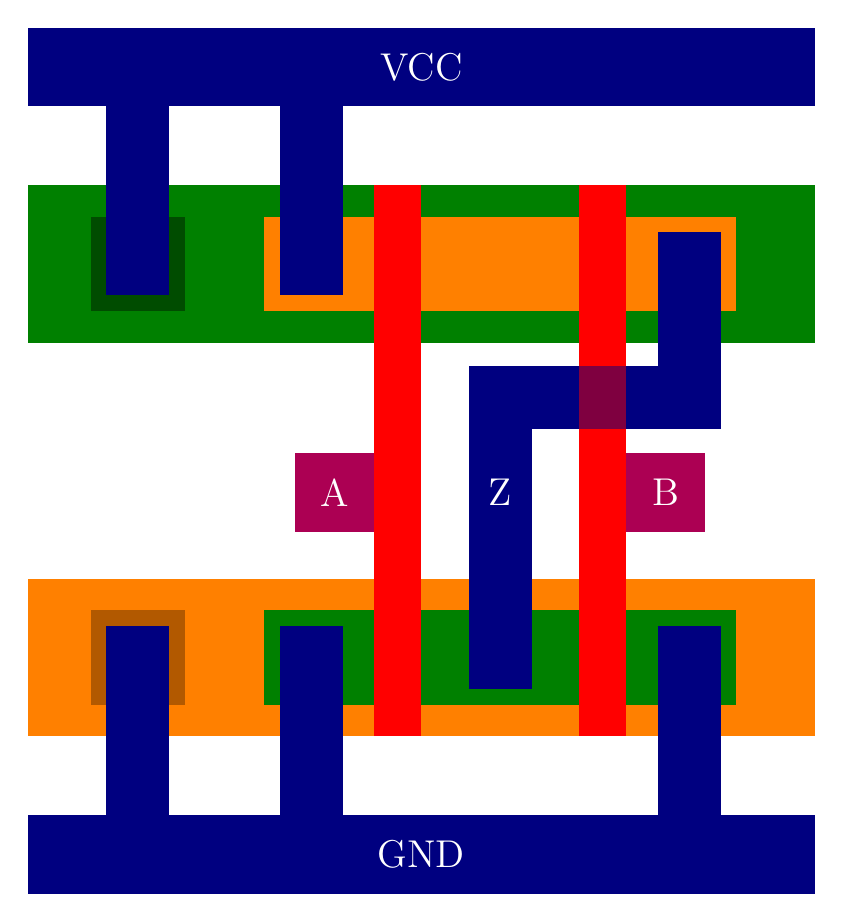
\begin{tikzpicture}
      \fill [fill=black!50!blue] (0, 0) rectangle (10, 1);
      \fill [fill=orange] (0, 2) rectangle (10, 4);
      \fill [fill=black!30!orange] (0.8, 2.4) rectangle (2.0, 3.6);
      \fill [fill=black!50!green] (3.0, 2.4) rectangle (9.0, 3.6);
      \fill [fill=black!50!blue] (1, 0.8) rectangle (1.8, 3.4);
      \fill [fill=black!50!blue] (3.2, 0.8) rectangle (4, 3.4);
      \fill [fill=black!50!blue] (8, 0.8) rectangle (8.8, 3.4);

      \fill [fill=black!50!blue] (0, 10) rectangle (10, 11);
      \fill [fill=black!50!green] (0, 7) rectangle (10, 9);
      \fill [fill=black!70!green] (0.8, 7.4) rectangle (2.0, 8.6);
      \fill [fill=orange] (3.0, 7.4) rectangle (9.0, 8.6);
      \fill [fill=black!50!blue] (1, 10.2) rectangle (1.8, 7.6);
      \fill [fill=black!50!blue] (3.2, 10.2) rectangle (4, 7.6);
      \fill [fill=black!50!blue] (8, 8.4) rectangle (8.8, 5.9);
      \fill [fill=black!50!blue] (5.6, 5.9) rectangle (8.8, 6.7);
      \fill [fill=black!50!blue] (5.6, 6.7) rectangle (6.4, 2.6);

      
      \fill [fill=red] (4.4, 2) rectangle (5.0, 9);
      \fill [fill=blue!10!purple] (3.4, 4.6) rectangle (4.4, 5.6);
      \fill [fill=red] (7, 2) rectangle (7.6, 9);
      \fill [fill=blue!10!purple] (7.6, 4.6) rectangle (8.6, 5.6);

      \fill [fill=black!50!blue, fill opacity=0.5] (7, 5.9) rectangle (7.6, 6.7);
      
      \node[white] at (5, 0.5) {\large GND};
      \node[white] at (5, 10.5) {\large VCC};
      \node[white] at (3.9, 5.1) {\large A};
      \node[white] at (8.1, 5.1) {\large B};
      \node[white] at (6, 5.1) {\large Z};
    \end{tikzpicture}
  \end{center}

  \item The answer is the figure below. \\
  \begin{center}
    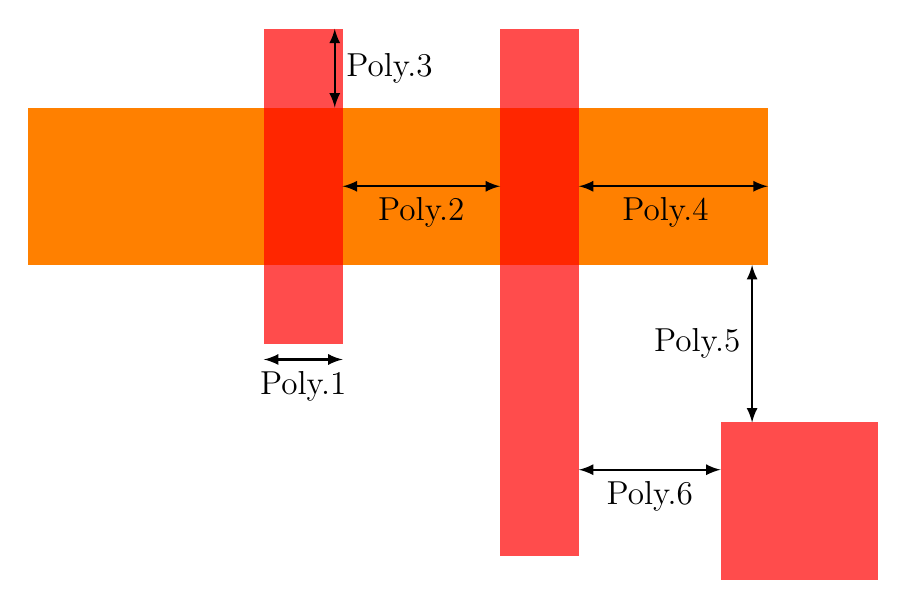
\begin{tikzpicture}
      \fill[fill=orange] (-2, 0) rectangle (7.4, 2);
      \fill[fill=red, fill opacity=0.7] (1, 3) rectangle (2, -1);
      \fill[fill=red, fill opacity=0.7] (4, 3) rectangle (5, -3.7);
      \fill[fill=red, fill opacity=0.7] (6.8, -2) rectangle (8.8, -4);

      \draw[latex-latex, thick] (1, -1.2) -- (2, -1.2);
      \node[below] at(1.5, -1.2) {Poly.1};
      \draw[latex-latex, thick] (2, 1) -- (4, 1);
      \node[below] at(3, 1) {Poly.2};
      \draw[latex-latex, thick] (1.9, 3) -- (1.9, 2);
      \node[right] at(1.9, 2.5) {Poly.3};
      \draw[latex-latex, thick] (5, 1) -- (7.4, 1);
      \node[below] at(6.1, 1) {Poly.4};
      \draw[latex-latex, thick] (7.2, 0) -- (7.2, -2);
      \node[left] at(7.2, -1) {Poly.5};
      \draw[latex-latex, thick] (5, -2.6) -- (6.8, -2.6);
      \node[below] at(5.9, -2.6) {Poly.6};
      
    \end{tikzpicture}
  \end{center}

\end{enumerate}

\end{document}

